
\section{Results}
\label{sec:experiment_results}

This section gives the results of the experiments listed in Section \ref{sec:experiment_plan}, which are analyzed further in Chapter \ref{ch:analysis}.



\begin{table}[h]
	\begin{tabular}{ll}
		\textbf{Adult} & \textbf{Error rate} \\
		Our optimal result (Local model, e=1.0, 10 peer)                  & 0.157 \\
		High privacy, few peers($\epsilon$=0.1, 50 peers)				  & 0.163  \\
		Aggregated model												  & 0.185 \\
		Ensemble model													  &	0.165
	\end{tabular}
	\caption{Table with baseline results from the Adult Dataset}
	\label{tab:baseline_class_results_adult}
\end{table}

%testing range of epsilon to see expected behavior
\todo[inline]{Consider rerunning this experiment without local model}
\begin{figure}[H]
	\centering
	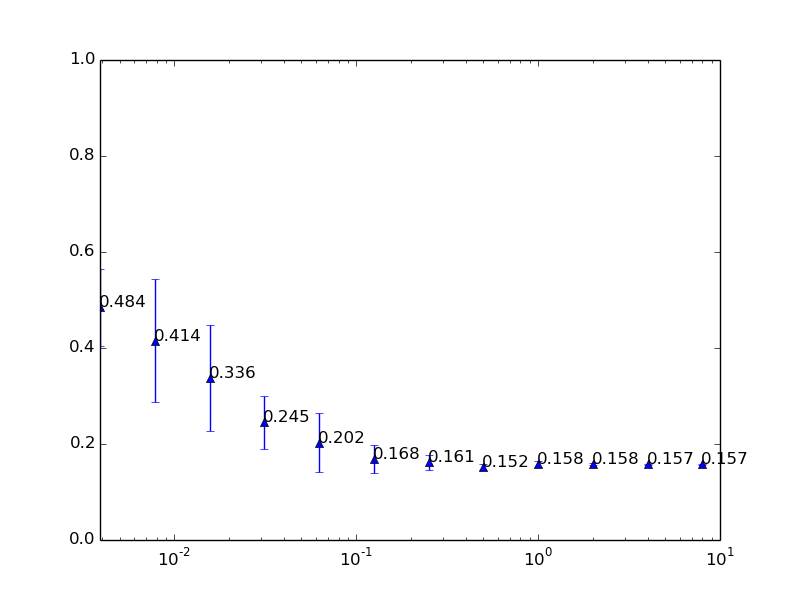
\includegraphics[width=\textwidth]{fig/spambase/eps2e-8-2e8,budg=eps,peers10,groups10,reg2e-2-data368-pubAll-spam-baseline-testset}
	\caption{$\epsilon = [10^{-3}, 10^{3}], \lambda = 2^{-4}$, 50 peers, 1 aggregation}
	\label{fig:epsilon_big_range}
\end{figure}

%testing range of regularization in various settings to validate presence of expected behavior
\begin{figure}[h!]
	\centering
	\begin{minipage}{.49\linewidth}
		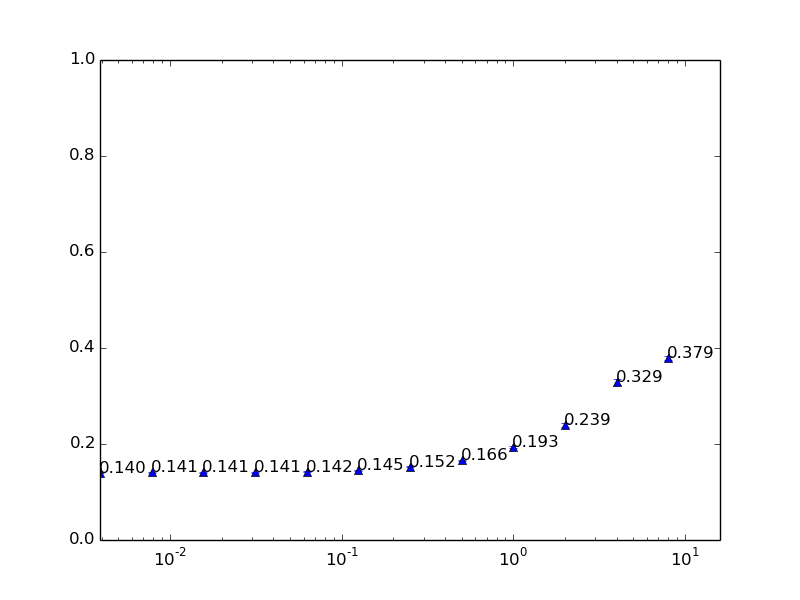
\includegraphics[width=\linewidth]{fig/spambase/eps2e10,budg=eps,peers10,groups10,reg2e-8-2e3-data368-pubAll-spam-baseline-testset}
		\captionof{figure}{$\epsilon = 2^{10}, \lambda = [2^{-8}, 2^{3}]$, 10 peers, 1 aggregation}
		\label{fig:regularization_extremelyhighepsilon}
	\end{minipage}
	\hspace{.001\linewidth}
	\begin{minipage}{.49\linewidth}
		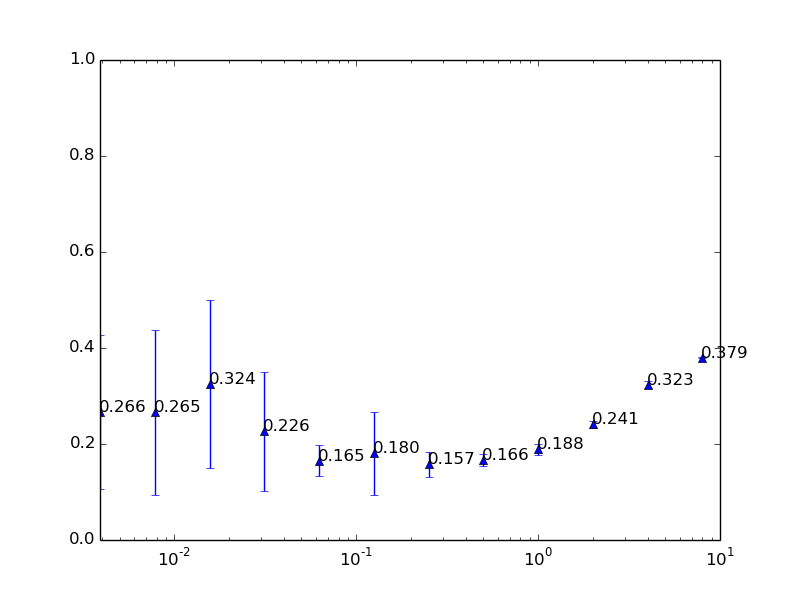
\includegraphics[width=\linewidth]{fig/spambase/eps0.1,budg=eps,peers10,groups10,reg2e-8-2e3-data368-pubAll-spam-baseline-testset}
		\captionof{figure}{$\epsilon = 0.1, \lambda = [2^{-8}, 2^{3}]$, 10 peers, 1 aggregation}
		\label{fig:regularization_normalepsilon}
	\end{minipage}
	\begin{minipage}{.49\linewidth}
		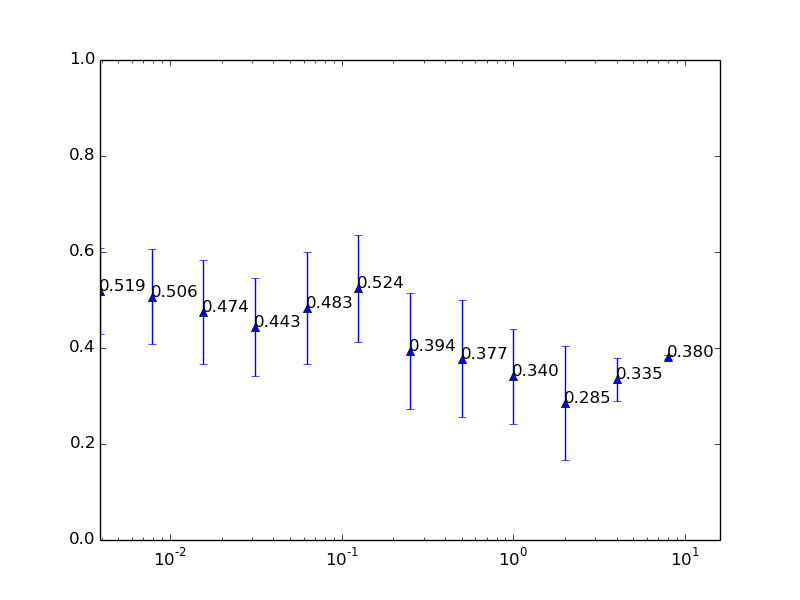
\includegraphics[width=\linewidth]{fig/spambase/eps0.01,budg=eps,peers10,groups10,reg2e-8-2e3-data368-pubAll-spam-baseline-testsetmean}
		\captionof{figure}{$\epsilon = 0.01, \lambda = [2^{-8}, 2^{3}]$, 10 peers, 1 aggregation}
		\label{fig:regularization_lowepsilon}
	\end{minipage}
\end{figure}

%figures showing the effect of data amounts in various combinations of models

\begin{figure}[h!]
	\centering
	\begin{minipage}{.49\linewidth}
		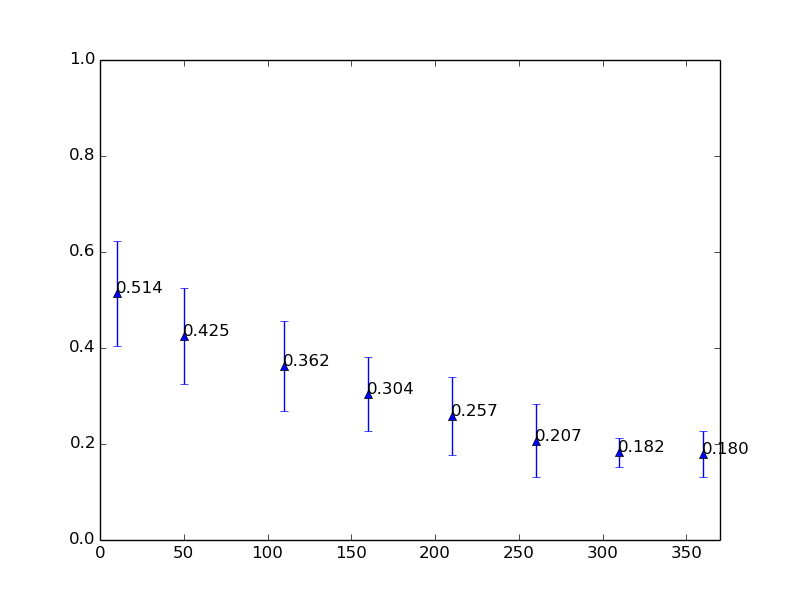
\includegraphics[width=\linewidth]{fig/spambase/eps0.1,budg=eps,peers10,groups10,reg2e-2-pubAll-spam-baseline-data10-360-testset-withoutlocalmodel}
		\captionof{figure}{$\epsilon = 0.1, \lambda = 2^{-2}$, 10 peers, 1 aggregations. Aggregated model only.}
		\label{fig:data_limit_test_withoutlocalmodel}
	\end{minipage}
	\hspace{.001\linewidth}
	\begin{minipage}{.49\linewidth}
		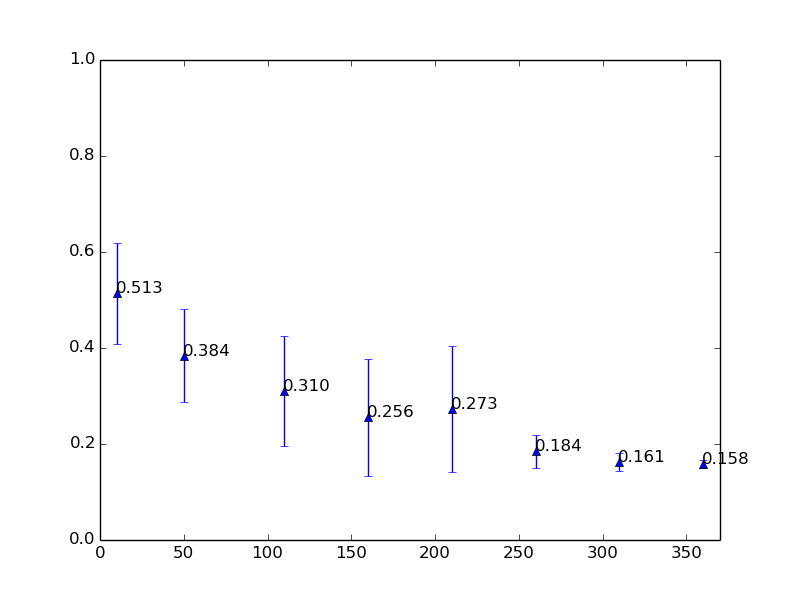
\includegraphics[width=\linewidth]{fig/spambase/eps0.1,budg=eps,peers10,groups10,reg2e-2-pubAll-spam-baseline-data10-360-testset-withlocalmodel}
		\captionof{figure}{$\epsilon = 0.1, \lambda = 2^{-2}$, 10 peers, 1 aggregation. Aggregated and local model.}
		\label{fig:data_limit_test_withlocalmodel}
	\end{minipage}
	\begin{minipage}{.49\linewidth}
		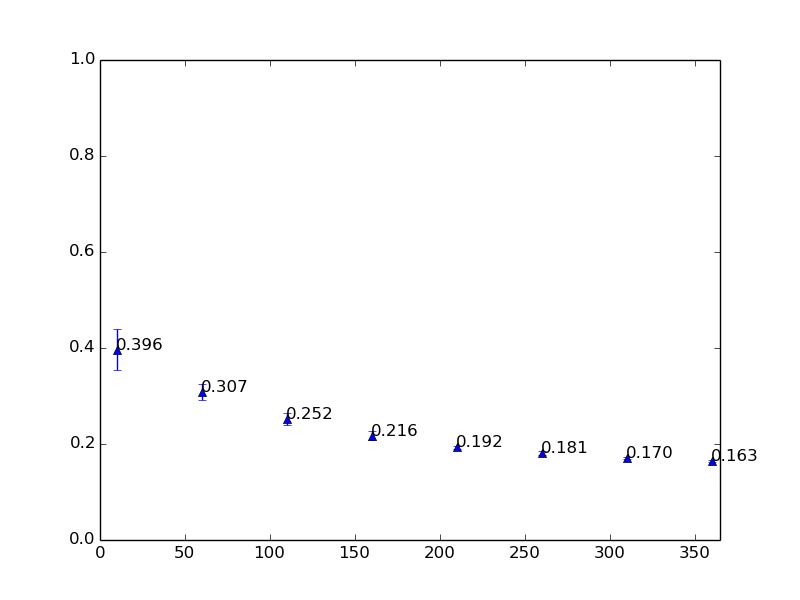
\includegraphics[width=\linewidth]{fig/spambase/eps0.1,budg=eps,peers10,groups10,reg2e-2-pubAll-spam-baseline-data10-360-testset-localmodelonly}
		\captionof{figure}{$\lambda = 2^{-2}$, 10 peers, local model only.}
		\label{fig:data_limit_test_localmodelonly}
	\end{minipage}
\end{figure}

%result of testing constant group size with ever larger number of peers
\todo[inline]{make Effect of peer numbers into a simple table row showing min/max instead}
\begin{figure}[h]
	\centering
	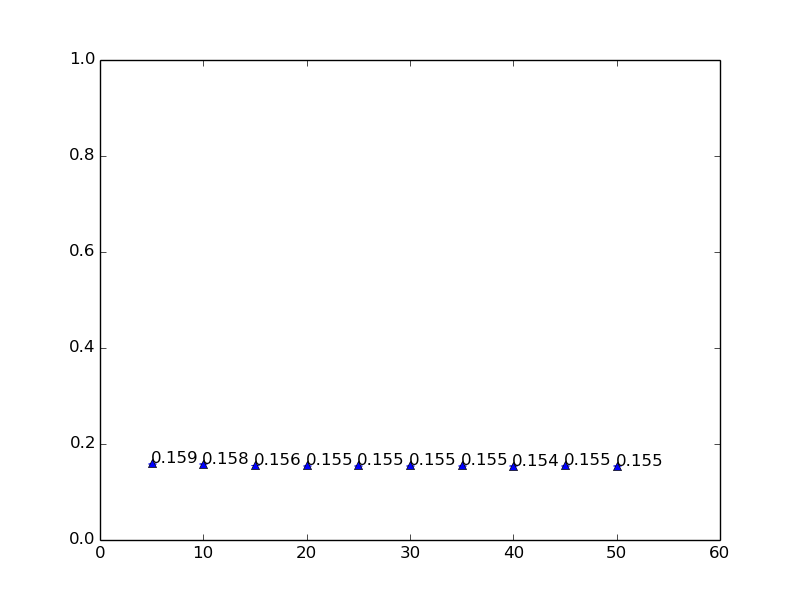
\includegraphics[width=\textwidth]{fig/adult/eps1.0,budg=eps,peers5-55,groups5,reg2e2-data500-pubAll-adult-groupbypeerverification-3-testsetmean}
	\caption{Effect of peer numbers. Group size: 50. Publishing: All. Data: 500}
	\label{fig:peer_range_constant_group}
\end{figure}


%figure showing the presence of variance among peers 
\todo[inline]{replace variance table with numbers from recent, properly CVed runs. ALSO, add std.dev. of std dev. :)}
\begin{table}[h]
	\centering
	\caption{Variance among peers, Adult}
	\label{table:peer_variance_adult}
	\begin{tabular}{|l|l|l|}
		\textbf{Model}                  & \textbf{Mean error} & \textbf{Peer std. dev.} \\
		\hline
		Local, no privacy      & 0,175 & 0.006 \\
		Aggregated, d. privacy & 0,158 & 0.000	 \\
		Ensemble with both & 0.166 & 0.002 \\
	\end{tabular}
\end{table}      

\begin{figure}[h]
	\centering
	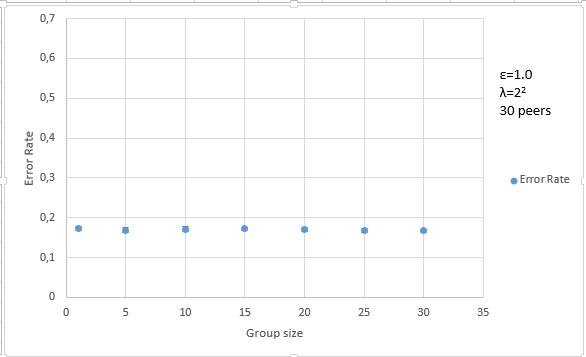
\includegraphics[width=\textwidth]{fig/adult/GroupSizeTest}
	\caption{Effect of Aggregation Group Sizes.}
	\label{fig:results_group_sizes}
\end{figure}

%add - some result comparing difference between party and all publishing


%add - some result showing what happens when group sizes change - maybe combined with the above


\begin{figure}[h]
	\centering
	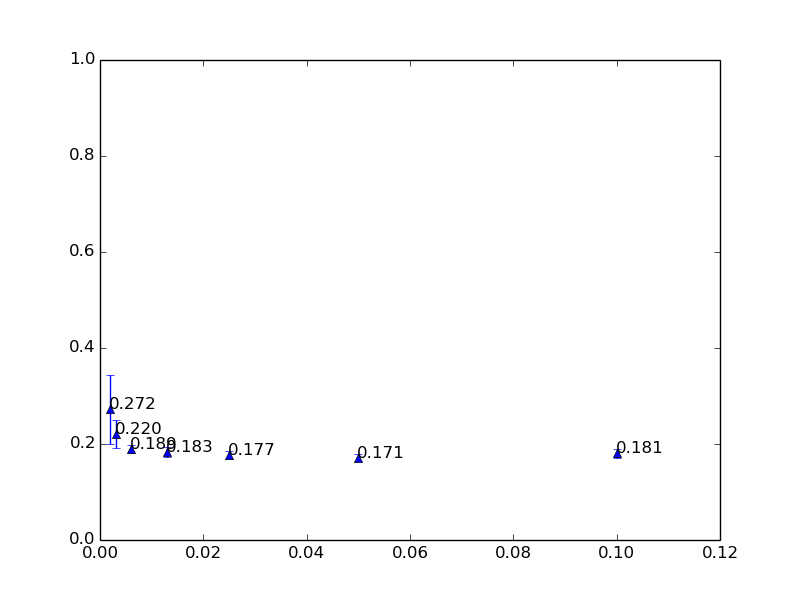
\includegraphics[width=\textwidth]{fig/adult/eps0.1,bud0.1div1-64,peers10,groups2,reg2e2-pubAll-groupsizetest-withoutlocal-data200-adultmean}
	\caption{Effect of Privacy Budgeting.}
	\label{fig:results_privacy_budget}
\end{figure}


%add - some result showing what happens when the amount of privacy budget used is changed - possibly considering all vs party also here


\cleardoublepage